\documentclass{article}
\usepackage[utf8]{inputenc}
\usepackage{amsmath}
\usepackage{graphicx}
\usepackage{float}
\usepackage[romanian]{babel}

\title{Referat: Determinarea Constantei Rydberg}
\author{Nicolas Dumitru}

\begin{document}

\maketitle

\section{Scopul lucrării}
Determinarea constantei implicate în seriile spectrale ale atomilor hidrogenoizi.

\section{Teoria lucrării}
Atomii fiecărui element chimic emit, atunci când sunt excitaţi (de exemplu într-o
descărcare în gaz), un spectru optic caracteristic de radiaţii, astfel că fiecare element poate fi
identificat după spectrul său. Aceasta este esenţa analizei spectrale calitative. De asemenea,
atomii pot fi excitaţi prin absorbţie de radiaţie, spectrul de absorbţie fiind identic cu cel de
emisie. Spectrele elementelor chimice sunt cu atât mai complicate, cu cât numărul lor de ordine
Z este mai mare. Spectrele optice ale atomilor sunt datorate electronilor optici, adică
electronilor ce se găsesc pe orbita periferică.

Spectroscopiştii experimentatori au stabilit că toate liniile din diferitele serii spectrale
ale atomului de hidrogen pot fi descrise printr-o relaţie generală care dă lungimea de undă a
liniilor spectrale /1-4/:
\begin{equation}
	\frac{1}{\lambda_{mn}} = \tilde{\nu}_{mn} = T(m) - T(n) = R_H \left( \frac{1}{m^2} - \frac{1}{n^2} \right)
\end{equation}

unde n şi m sunt numere întregi, T(m) şi T(n) sunt termeni spectrali, iar $R_H$ este constanta
Rydberg. $\tilde{\nu}{mn}$ este numărul de undă (cunoscut şi ca frecvenţă spaţială), definit ca inversul
lungimii de undă $\lambda{mn}$. Relaţia (1) este formularea matematică a principiului de combinare
Rydberg-Ritz: toate frecvenţele (sau numerele de undă) ale atomului de hidrogen pot fi scrise
ca diferenţa a doi termeni spectrali iar dacă există în spectru frecvenţele (spaţiale) $\tilde{\nu}{mk}$
şi $\tilde{\nu}{nk}$, atunci există de asemenea diferenţa lor $\tilde{\nu}_{mn}$.

I. Atomul se poate afla într-un şir discret de stări staţionare, determinate de şirul discret
$E_1$, $E_2$, \ldots, $E_n$ \ldots de valori ale energiei totale. În aceste stări atomul nici nu emite, nici nu
absoarbe energie.

II. Energia atomului poate varia discontinuu, prin trecerea de la o stare staţionară de
energie totală $E_m^0$ la altă stare staţionară de energie totală $E_m$. Frecvenţa fotonului absorbit
sau emis este dată de relaţia:
\begin{equation}
	\nu_{mn} = \frac{\left| E_m^0 - E_m\right|}{h}
\end{equation}

procesul de absorbţie având loc în cazul în care electronul trece de pe o orbită mai apropiată de
nucleu pe una mai depărtată, iar emisia atunci când parcurge drumul invers.

III. Mărimea momentului cinetic al electronului pe orbitele circulare permise în jurul
nucleului trebuie să fie egală cu un număr întreg de $\hbar$:
\begin{equation}
	M = mvr = n\hbar
\end{equation}

unde $\hbar = \frac{h}{2\pi}$ este constanta lui Planck redusă, h este constanta lui Planck iar n se numeşte
număr cuantic principal şi poate lua valorile n = 1, 2, 3,....

Astfel, considerând modelul planetar al atomului cu nucleul (protonul) imobil, se obţine
că energia totală $E_n$ (compusă din energia cinetică a electronului în mişcarea sa în jurul
nucleului şi energia electrostatică de interacţie coulombiană nucleu-electron) pe orbita n este
cuantificată:
\begin{equation}
	E_n = -\frac{me^4}{8\epsilon_0^2h^2}\frac{1}{n^2}
\end{equation}

unde m este masa electronului, e este sarcina electronului şi $\epsilon_0$ este permitivitatea electrică a
vidului.

Cea mai scăzută energie a atomului de hidrogen (numită şi stare fundamentală)
corespunde numărului numărului cuantic n = 1 şi are valoare de –13,6 eV. Ionizarea atomului
de hidrogen, adică spargerea lui într-un nucleu şi un electron corespunde unei depărtări practic
infinite dintre aceste particule, energia minimă a acestui sistem fiind zero. Energia minimă
necesară pentru a ioniza atomul de hidrogen aflat în starea fundamentală se numeşte energie de
ionizare şi are valoarea de 13,6 eV.

În mecanica cuantică energia atomului de hidrogen, expresia (4), se află prin integrarea
ecuaţiei Schrödinger, fără a se mai introduce condiţia (3).

Energia totală a atomului de hidrogen este negativă (ecuaţia (4)), ceea ce exprimă
faptul că electronul se află legat în câmpul electromagnetic al nucleului.

Folosind relaţiile (2) şi (4) se obţine:
\begin{equation}
	\frac{1}{\lambda_{mn}} = \frac{me^4}{8\epsilon_0^2h^3c}\left(\frac{1}{m^2} - \frac{1}{n^2}\right)
\end{equation}

care comparată cu (1), conduce la relaţia:
\begin{equation}
	R_H = \frac{me^4}{8\epsilon_0^2h^3c}
\end{equation}

expresie obţinută în cazul modelului în care s-a considerat protonul imobil.

Din relaţia (2) pot fi găsite toate lungimile de undă ale liniilor diferitelor serii spectrale
ale hidrogenului. O serie spectrală reprezintă totalitatea liniilor spectrale care au un nivel
energetic de bază comun (fig.1).

Astfel există seria Lyman (ultraviolet) la care nivelul energetic comun este
corespunzător lui m=1 (în relaţia (5)) și $n \geq 2$; seria Balmer (vizibil) la care m = 2 şi $n \geq 3$;
seria Paschen la care m = 3 şi $n \geq 4$ iar liniile spectrale au lungimile de undă corespunzătoare
radiaţiilor din infraroşu etc.

În cazul seriei Balmer, relaţia (1) devine:
\begin{equation}
	\frac{1}{\lambda_n} = R_H\left(\frac{1}{2^2} - \frac{1}{n^2}\right) \quad \text{unde } n=3,4,5,6,\ldots
\end{equation}

de unde rezultă constanta Rydberg:
\begin{equation}
	R_H = \frac{1}{\lambda_n}\cdot\frac{n^2}{1-\frac{4}{n^2}}
\end{equation}

\begin{figure}
	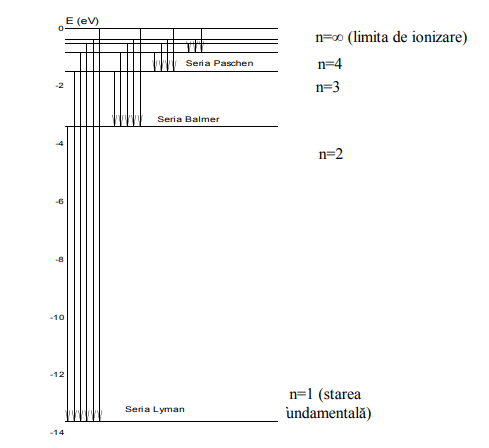
\includegraphics[width=0.5\linewidth]{serii-spectrale.png}
	\caption{Serii spectrale}
\end{figure}
\begin{figure}
	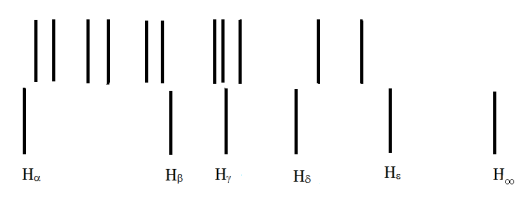
\includegraphics[width=0.5\linewidth]{spectrograme.png}
	\caption{Spectrogramele pentru hidrogen și mercur înregistrate pe aceeași
		placă fotografică}
\end{figure}

\end{document}
